\section{Deployment Diagram}\label{sec:sprint2-deploymentdia}
In \autoref{sec:sprint1-architecture} the different components of the system were introduced in \autoref{fig:architecture}.
A deployment diagram is constructed in this section in order to further elaborate on the different components.
The deployment diagram can be seen on \autoref{fig:sprint2-deployment}.
\begin{figure}[H]
    \centering
    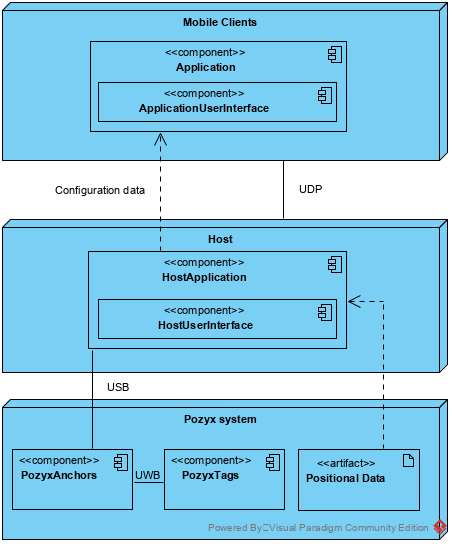
\includegraphics[width=0.6\linewidth]{deploymentdiagram.png}
    \caption{A deployment diagram for the system.}
    \label{fig:sprint2-deployment}
\end{figure}
\noindent
A deployed system will contain three nodes:
\begin{itemize}
    \item Pozyx system
    \item Host
    \item Mobile Clients
\end{itemize}
Nodes are represented by cubes, and are entities that execute components.
The Pozyx system node contains two components.
These are the anchors and the tags needed to generate positional data with the Pozyx hardware.
The system contains multiples of anchors and tags.
These Pozyx components generate artifacts in terms of positional data for the location of the players and the ball.
Anchors and tags are associated through a UWB connection in order to generate these artifacts.
The host node is dependent on the positional data artifact, as the component receives the positional data and transforms it for communication.
Positional data is transferred from the Pozyx system to the host through a USB association.
One anchor is associated with the host application, and this anchor is responsible for collecting data from all tags.
The host application component contains a user interface component, which is the interface that the person using the host component will interact with, in the form of a console application for the early version of the system.
The host node is associated with the clients through a UDP connection in order to communicate both the positional data and the configuration data to perform game setup.
As such, the mobile client application component is dependent on the host application component, since it requires the configuration data.
The mobile clients also contain user interface components, which is how the users interact with that part of the system.
This user interface is the virtual playing field generated in Unity that the users view in the headset.
